\documentclass{article}
\usepackage{tikz}
\usepackage[margin=1in]{geometry}
\usepackage{ifthen}
\usepackage{helvet}
\renewcommand{\familydefault}{\sfdefault}

\begin{document}

% Header with blank fields
\begin{center}
    \LARGE \textbf{Combustion Residue Mapping Sheet} \\[2ex]
    \large \textbf{Project:} \underline{\hspace{8cm}} \\[1ex]
    \large \textbf{Date:} \underline{\hspace{3.5cm}} \hspace{2cm}
    \textbf{Researcher:} \underline{\hspace{4cm}}
\end{center}

\vspace{1cm}

% Oven map
\begin{center}
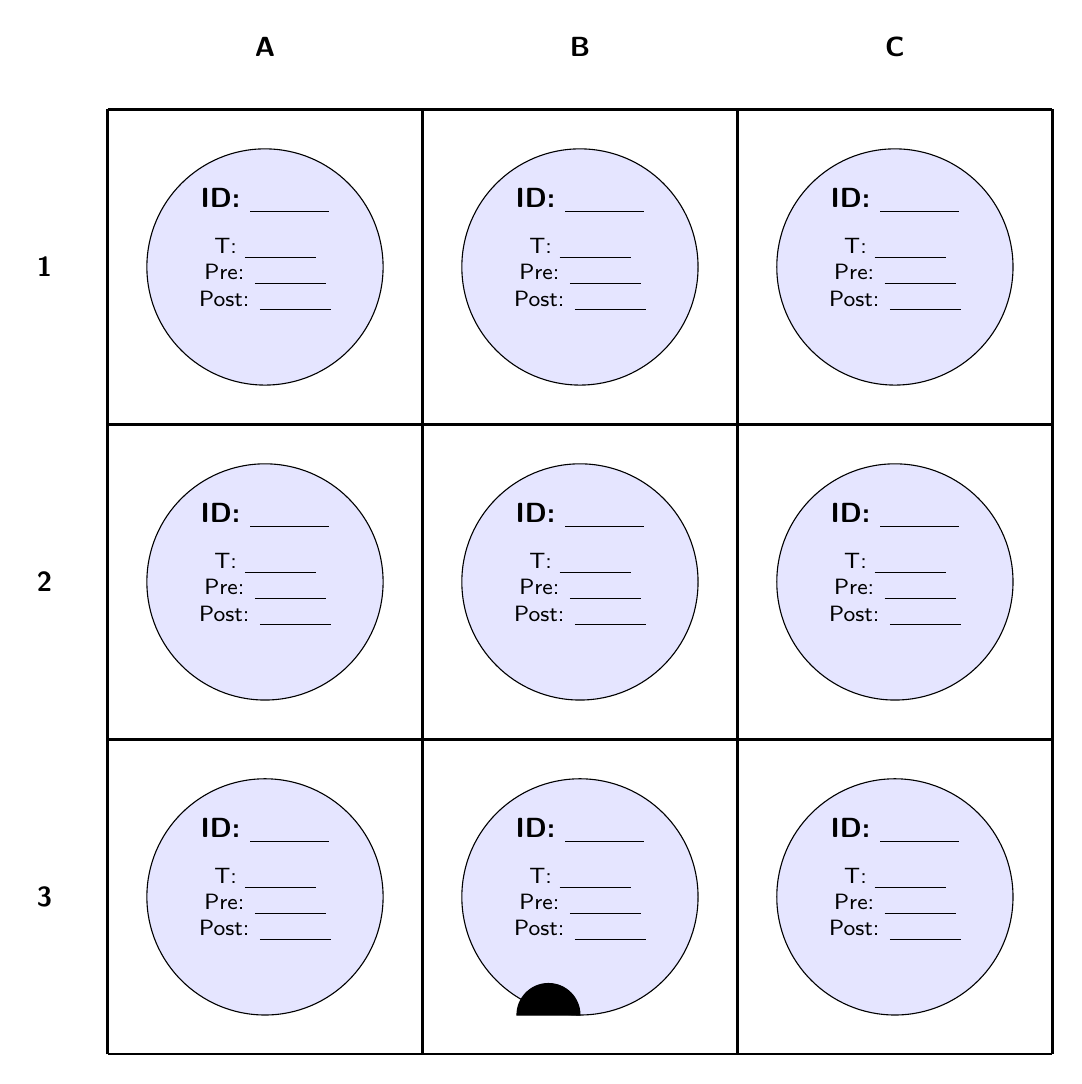
\begin{tikzpicture}[scale=2]
  \def\cellsize{2}
  \def\n{3}

  % Draw grid
  \foreach \x in {0,...,\n} {
    \draw[thick] (0,\x*\cellsize) -- (\n*\cellsize,\x*\cellsize);
    \draw[thick] (\x*\cellsize,0) -- (\x*\cellsize,\n*\cellsize);
  }

  % Sample circles and data
  \foreach \i/\j in {
    0/2, 1/2, 2/2,
    0/1, 1/1, 2/1,
    0/0, 1/0, 2/0}
  {
    \pgfmathsetmacro{\x}{\i*\cellsize + \cellsize/2}
    \pgfmathsetmacro{\y}{\j*\cellsize + \cellsize/2}

    % Draw sample circle
    \draw[fill=blue!10] (\x,\y) circle (0.75cm);

    % Orientation marker
    \ifthenelse{\i=1 \AND \j=0}{
        \draw[fill=black] (\x,\y-0.75) arc[start angle=0, end angle=180, radius=0.2cm] -- cycle;
    }{}

    % ID label
    \node[align=center, font=\normalsize] at (\x,\y+0.42) {\textbf{ID: \underline{\hspace{1cm}}}};

    % T/Pre/Post values
    \node[align=center, font=\footnotesize] at (\x,\y-0.05) {
        T: \underline{\hspace{0.9cm}}\\
        Pre: \underline{\hspace{0.9cm}}\\
        Post: \underline{\hspace{0.9cm}}
    };
  }

  % Axis labels
  \foreach \i in {0,...,2} {
    \node at (-0.4, \i*\cellsize + \cellsize/2) {\textbf{\the\numexpr3-\i}};
    \node at (\i*\cellsize + \cellsize/2, \n*\cellsize + 0.4) {\textbf{\char\numexpr65+\i}};
  }

\end{tikzpicture}
\end{center}

\vspace{0.5cm}
\noindent \textbf{Legend:} \\ 
T = Tare weight (g), Pre = Pre-combustion weight (g), Post = Post-combustion weight (g)

\end{document}
